In the classical simulations, the state preparation would require to produce a random qubit pure state first, and then to compute the corresponding Bloch vector to be used later by Alice. 

In the prepare-and-measure scenario, Alice uses the Bloch vector representation of the qubit's pure state, and Bob's POVMs,  proportional to rank-1 projectors, are expressed as the outer product of the associated Bloch vectors. In the Bell scenario, Alice also uses the Bloch vector corresponding to the local projective measurement projectors. In addition, in all these protocols, Alice and Bob share two random normalized vectors $\vec{\lambda}_1, \vec{\lambda}_2 \in \mathbb{R}^{3}$, which must be uniformly and independently distributed on the unit sphere $S_2$, which is analogous to generate random Bloch vectors in the Bloch sphere. Given the fact that the classical probabilities obtained with the different protocols must be equivalent to the quantum probabilities for any state and POVM measure, and that generating a true shared randomness is a fundamental element of the classical protocols, it is of key importance to be able prepare random normalized vectors uniformly distributed along the unit radius sphere $S_2$. Hence, the randomized qubit state preparation in the form of Bloch vectors is not only the building block for the state preparation itself, but plays also a critical role in the measurement construction and the shared randomness creation.

To produce a random qubit pure state we should obtain a random unitary matrix and then apply the unitary transformation to the zero qubit state, resembling the time evolution of a qubit from a zero initial state. The random unitary matrix can be generated by just building a matrix of normally distributed complex numbers, and then apply the Gram-Schmidt QR decomposition to orthogonalize the matrix, see \cite{ozols2009}, \cite{zyczkowski1994}. 

The resulting random qubit state distribution can be validated using the corresponding Bloch vector distribution along the unit radius sphere. A tessellation scheme called HEALPix \cite{healpix}, which produces a hierarchical and equal-area iso-latitude pixelation of a sphere, could be used to show that the random Bloch vectors are uniformly and independently distributed in the Bloch sphere. Given that each pixel in HEALPix covers the same surface area as every other pixel (see Figure \ref{fig:healpix_sphere}), we can group the Bloch vector distribution along the different pixel indices (see Figure \ref{fig:healpix_numbering}), and check whether the resulting distribution is uniform as expected.

\begin{figure}[!ht]
\begin{center}
\centerline{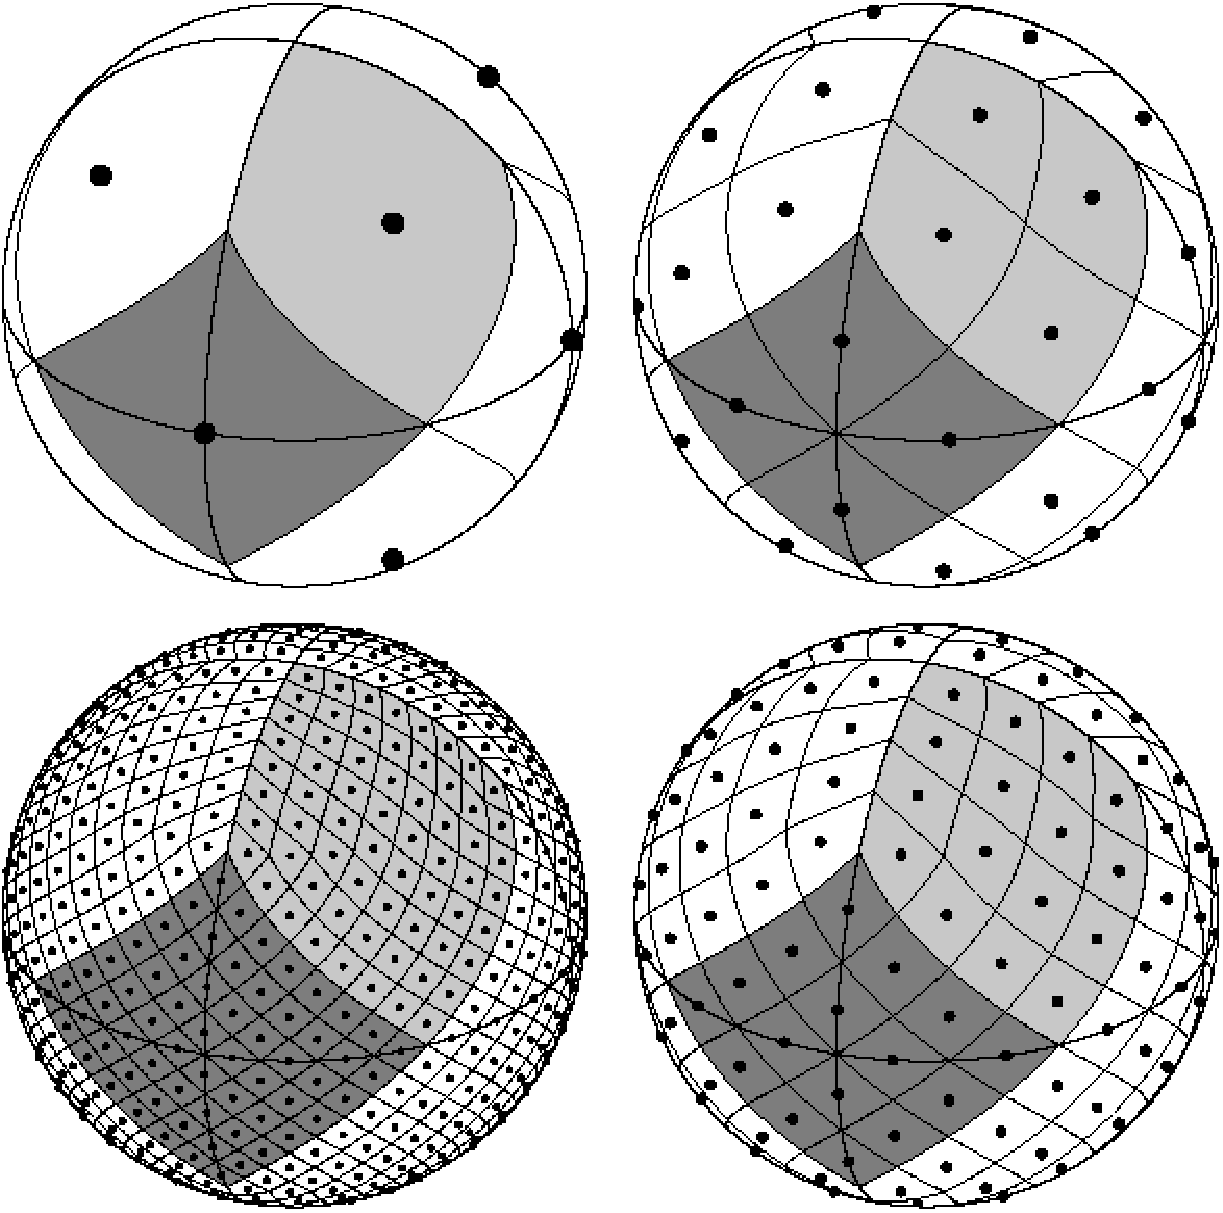
\includegraphics[height=5.5cm]{images/healpix4.pdf}}
\caption[Orthographic view of Healpix partition of the sphere]%
{\label{fig:healpix_sphere}%
Orthographic view of HEALPix partition of the sphere.}
\end{center}
\end{figure}

\begin{figure} [!ht]
\begin{center}
\centerline{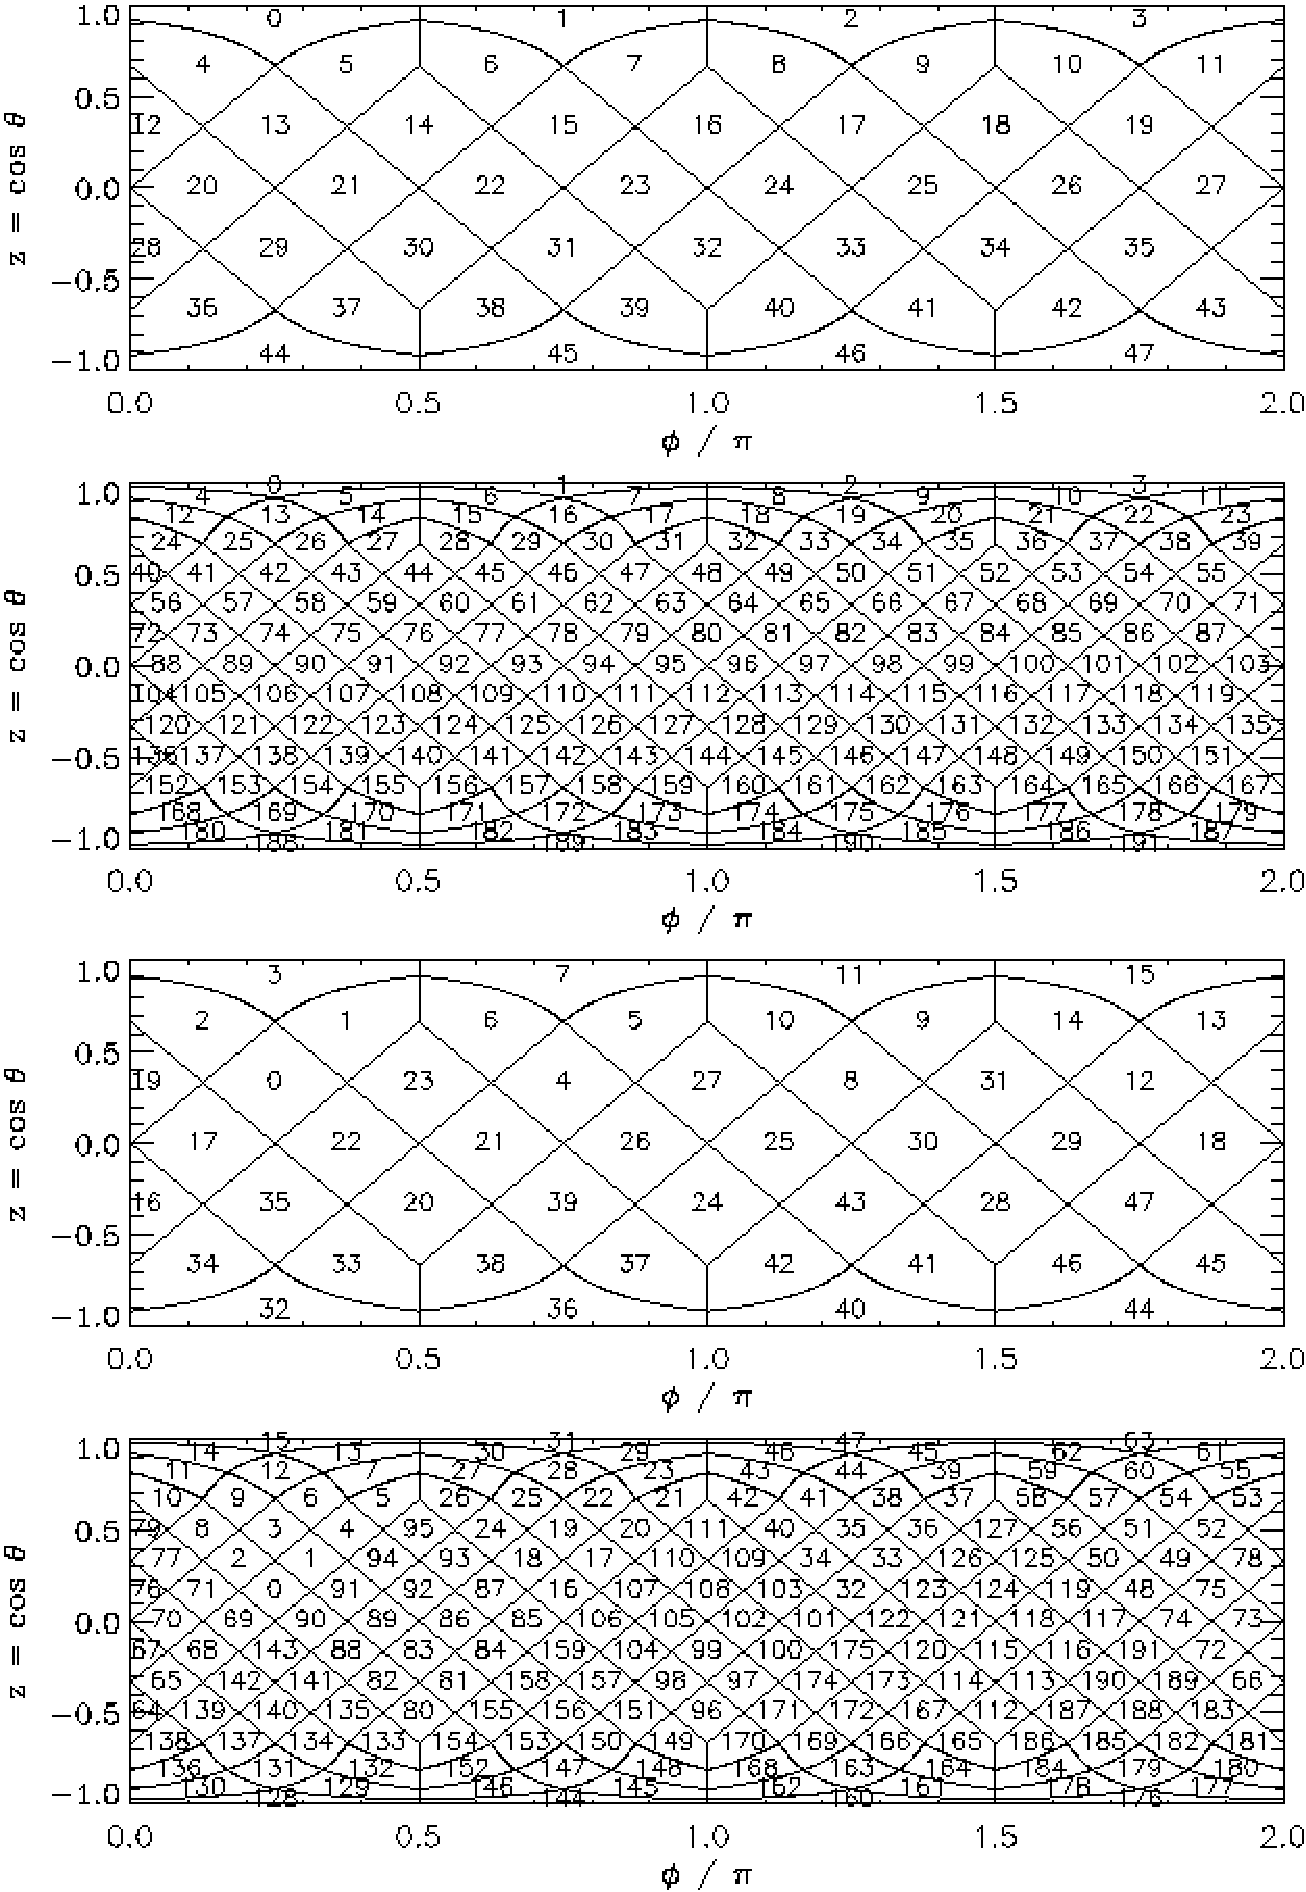
\includegraphics[height=10.5cm]{images/healpix2d.pdf}}
\caption[Cylindrical projection]%
{\label{fig:healpix_numbering}%
Cylindrical projection of the HEALPix division of a
sphere and two natural pixel numbering schemes (RING and NESTED). 
Both numbering schemes map the two dimensional 
distribution
of discrete area elements on a sphere into the one dimensional, 
integer pixel number array.
}
\end{center}
\end{figure}